\documentclass[11pt, letterpaper]{article}
\usepackage{amsmath, amssymb}
\usepackage{hyperref}
\usepackage{booktabs}
\usepackage{enumitem}
\usepackage{xcolor}
\usepackage{geometry}
\usepackage{fancyhdr}
\usepackage{titlesec}
\usepackage{tcolorbox}
\usepackage{graphicx}
\usepackage{parskip}
\usepackage{caption}
\geometry{margin=1in}

\definecolor{courseblue}{HTML}{002452}
\definecolor{coursegold}{HTML}{FABD0F}
\definecolor{coursered}{HTML}{B90E31}
\definecolor{lightblue}{HTML}{E8EEF7}
\definecolor{lightgold}{HTML}{FEF8E3}

\hypersetup{colorlinks=true,linkcolor=courseblue,urlcolor=coursered}
\tcbuselibrary{skins}
\newtcolorbox{guidancebox}{enhanced,colback=lightblue,colframe=courseblue,
  sharp corners,leftrule=4pt,left=6pt,right=6pt,top=4pt,bottom=4pt}
\newtcolorbox{notebox}{enhanced,colback=lightgold,colframe=coursegold,
  sharp corners,leftrule=4pt,left=6pt,right=6pt,top=4pt,bottom=4pt}

\pagestyle{fancy}\fancyhf{}
\fancyhead[L]{\small\textcolor{courseblue}{\textbf{CISC 473 --- Deep Learning | Fall 2026}}}
\fancyhead[R]{\small\textcolor{courseblue}{Midterm Report}}
\fancyfoot[C]{\small\thepage}
\renewcommand{\headrulewidth}{0.4pt}
\titleformat{\section}{\large\bfseries\color{courseblue}}{}{0em}{}[\titlerule]
\titleformat{\subsection}{\normalsize\bfseries\color{courseblue}}{}{0em}{}

\begin{document}

{\centering
  {\Large\textbf{CISC 473: Deep Learning --- Midterm Report}}\\[0.5em]
  {\large\textit{P08: Abstractive Summarization via Parameter-Efficient Fine-Tuning}}\\[0.4em]
  \textbf{Group Members:}\\
  Choo Wen Bin (20630085) (Project Lead) \quad
  Nai Junn Rong (20630086) (Research Lead)\\[0.3em]
  \textbf{GitHub:} \url{https://github.com/wenbin05/DeepLearningP08} \quad \textbf{Date:} October 17, 2026\\[0.4em]
  \rule{\linewidth}{0.4pt}
}

\section{Abstract}
Abstractive text summarization demands substantial computational and memory resources when adapting pre-trained sequence-to-sequence models through full fine-tuning. While Parameter-Efficient Fine-Tuning (PEFT) techniques like Low-Rank Adaptation (LoRA) dramatically reduce trainable parameter counts, standard practice applies adapters uniformly across all attention projections without considering functional module roles. In this project, we investigate how the architectural placement of LoRA adapters influences summarization performance, factual consistency, and cross-domain robustness in BART-base. To date, we have implemented the data preprocessing and evaluation pipeline for CNN/DailyMail and XSum, reproduced the published BART-base full fine-tuning baseline within $0.5\%$ ROUGE error, and established a budget-matched framework isolating encoder self-attention, decoder self-attention, and cross-attention adapters at exactly 147,456 trainable parameters (0.11\% of the model). Our preliminary results demonstrate that cross-attention LoRA achieves a ROUGE-1 score of $41.42 \pm 0.16$, capturing over 95\% of standard LoRA's performance while utilizing one-third of its parameter budget and substantially outperforming encoder-only adaptation ($39.82 \pm 0.22$). In the second half of the semester, we will complete multi-seed evaluations across out-of-domain XSum data, execute the human factuality study, and deliver our final comparative analysis.

\section{Introduction and Problem Statement}
Abstractive summarization compresses lengthy source documents into fluent, salient, and factually accurate summaries. Pre-trained sequence-to-sequence Transformers such as BART~\cite{lewis2020bart} achieve high ROUGE scores by leveraging bidirectional encoder representations coupled with autoregressive decoder generation. However, conventional adaptation requires updating all 139.4 million parameters in BART-base, incurring steep computational overhead and high storage requirements when maintaining separate checkpoints for multiple domains or tasks. Parameter-efficient fine-tuning (PEFT) methods, particularly Low-Rank Adaptation (LoRA)~\cite{hu2022lora}, circumvent this cost by freezing the pre-trained weights $W_0 \in \mathbb{R}^{d \times k}$ and injecting trainable rank-decomposition matrices $\Delta W = B A$.

\textbf{Scope Refinement and Changes Since Proposal.} In our initial proposal, we outlined extensive multi-factor ablations spanning various LoRA ranks ($r \in \{4, 8, 16\}$), target projection subsets ($Q, K, V, O$), and alternative PEFT paradigms (Prefix-Tuning). Following faculty feedback advising a more focused scope for a two-member team, we refined our investigation to prioritize the core architectural question: \textit{where} adaptation capacity should be allocated within an encoder-decoder model when total capacity is strictly controlled. Rather than conflating module placement with parameter volume, we exploit the structural symmetry of BART-base---wherein both the encoder and decoder contain 6 layers of identical hidden dimension ($d = 768$)---to fix the parameter budget to exactly 147,456 trainable parameters across all isolated placement variants.

\textbf{Research Question.} Under strictly matched trainable parameter budgets and identical training conditions, how does the architectural placement of LoRA adapters (encoder self-attention vs. decoder self-attention vs. encoder-decoder cross-attention) govern summarization performance, factual consistency, and zero-shot cross-domain generalization?

\section{Related Work (Updated)}
Parameter-efficient fine-tuning for conditional text generation has evolved rapidly, transitioning from uniform parameter perturbation to structural and capacity-aware allocation.

\textbf{Parameter-Efficient Sequence-to-Sequence Modeling.} Large-scale pre-training of sequence-to-sequence architectures, exemplified by BART~\cite{lewis2020bart}, established denoising objectives as the foundation for modern summarization. While full fine-tuning updates all parameters, Prefix-Tuning~\cite{li2021prefix} introduced continuous virtual prefix vectors prepended to attention keys and values, preserving frozen model weights while achieving competitive generation on XSum with under 2\% parameter overhead. Concurrently, LoRA~\cite{hu2022lora} demonstrated that task-specific parameter updates exhibit low intrinsic dimensionality, parametrizing weight updates via low-rank matrices $\Delta W = BA$. In their foundational work, Hu et al. observed that adapting attention query and value projections suffices for autoregressive language models. However, their primary benchmarks focused on decoder-only models, leaving the distinct functional components of encoder-decoder architectures unexamined.

\textbf{Non-Uniform Capacity Allocation and Layer Sensitivity.} Recognizing that uniform low-rank parameterization across all layers may be sub-optimal, recent research has explored dynamic allocation. AdaLoRA~\cite{zhang2023adalora} parameterizes weight matrices using singular value decomposition and iteratively prunes singular values based on importance scores, allocating higher rank to influential matrices. Similarly, WeightLoRA~\cite{veprikov2026weightlora} evaluates adapter significance during fine-tuning, demonstrating that adapters are not uniformly useful throughout BART. In a broader theoretical analysis, He et al.~\cite{he2022unified} established a unified framework connecting adapters, prefix tuning, and LoRA, proving that modification location directly shapes representation subspace alignment. Furthermore, Valipour et al.~\cite{valipour2023dylora} introduced DyLoRA to train models across a spectrum of ranks dynamically, showing that representation rank requirements differ sharply between early feature encoding and autoregressive token emission. While these methods demonstrate parameter non-uniformity, they optimize allocation dynamically via complex heuristics, leaving open the empirical question of how distinct, interpretable architectural blocks perform under an identical, static budget.

\textbf{Factual Consistency in Abstractive Summarization.} A known limitation of n-gram overlap metrics such as ROUGE-1, ROUGE-2, and ROUGE-L is their insensitivity to factual hallucinations. Kryscinski et al.~\cite{kryscinski2020evaluating} demonstrated that high-ROUGE summaries frequently introduce factual inconsistencies unsupported by the source text, proposing FactCC as a weakly supervised evaluation metric. Because FactCC's accuracy degrades when evaluated out-of-domain (e.g., dropping from 72.65\% on CNN/DailyMail to 54.11\% on XSum), human evaluation remains essential for reliable factuality assessment. Our study combines lexical ROUGE metrics with human evaluation to determine whether adapter placement influences factual hallucination rates.

\begin{center}
\small
\begin{tabular}{@{}llp{4.7cm}p{4.7cm}@{}}
\toprule
\textbf{Method} & \textbf{Year} & \textbf{Key Idea} & \textbf{Relation to Our Work} \\
\midrule
BART~\cite{lewis2020bart} & 2020 & Bidirectional encoder + autoregressive decoder seq2seq pre-training. & Primary backbone architecture for our summarization study. \\
LoRA~\cite{hu2022lora} & 2022 & Low-rank weight update factorization ($\Delta W = BA$). & Core PEFT mechanism evaluated across architectural placements. \\
Prefix-Tuning~\cite{li2021prefix} & 2021 & Virtual task-specific prefix vectors prepended to attention keys/values. & Baseline conditional conditioning approach for comparison. \\
AdaLoRA~\cite{zhang2023adalora} & 2023 & SVD-based parameterization with dynamic rank allocation. & Demonstrates non-uniform capacity importance; motivates explicit placement study. \\
Unified PEFT~\cite{he2022unified} & 2022 & Unified functional framework linking adapters, prefixes, and LoRA. & Theoretical grounding for structural placement effects. \\
DyLoRA~\cite{valipour2023dylora} & 2023 & Dynamic search of LoRA ranks during training. & Highlights layer-wise capacity sensitivity in generation tasks. \\
WeightLoRA~\cite{veprikov2026weightlora} & 2026 & Selectable LoRA units pruned during training. & Confirms adapter utility varies across BART layers. \\
FactCC~\cite{kryscinski2020evaluating} & 2020 & Factual-consistency classifier for abstractive summarization. & Highlights ROUGE limitations and justifies our human evaluation protocol. \\
\bottomrule
\end{tabular}
\captionof{table}{Comparative taxonomy of related work and foundational methods.}
\end{center}

\section{Methodology}
Our methodology enforces strict experimental consistency to guarantee that performance differences originate solely from adapter placement rather than training variations or capacity disparities.

\subsection{Model Architecture and Placement Isolation}
We use pre-trained \texttt{facebook/bart-base} as our backbone, which comprises an encoder with 6 Transformer layers and a decoder with 6 Transformer layers ($d_{\text{model}} = 768$, 16 attention heads, feed-forward dimension $d_{\text{ff}} = 3072$, totaling 139,420,416 parameters). For any weight matrix $W_0 \in \mathbb{R}^{d \times k}$, LoRA parameterizes the forward pass as:
\begin{equation}
h = W_0 x + \Delta W x = W_0 x + \frac{\alpha}{r} B A x
\end{equation}
where $A \in \mathbb{R}^{r \times k}$ is initialized from $\mathcal{N}(0, \sigma^2)$, $B \in \mathbb{R}^{d \times r}$ is initialized to zero, $r$ is the adaptation rank, and $\alpha$ is a scaling hyperparameter. We set $r = 8$ and $\alpha = 16$, targeting the query ($W_q$) and value ($W_v$) projections ($k = d = 768$). Each adapted projection introduces $2 \times 768 \times 8 = 12,288$ parameters.

We construct four distinct LoRA configurations:
\begin{enumerate}[leftmargin=*,itemsep=1pt]
  \item \textbf{Standard LoRA (All Attention):} Injects adapters into $W_q$ and $W_v$ across all 6 encoder self-attention, 6 decoder self-attention, and 6 decoder cross-attention blocks (18 attention layers total $\times 24,576 = 442,368$ trainable parameters, $0.32\%$ of the base model).
  \item \textbf{Encoder Self-Attention LoRA:} Adapts only \texttt{model.encoder.layers.*.self\_attn} ($6 \times 24,576 = 147,456$ trainable parameters, $0.11\%$).
  \item \textbf{Decoder Self-Attention LoRA:} Adapts only \texttt{model.decoder.layers.*.self\_attn} ($6 \times 24,576 = 147,456$ trainable parameters, $0.11\%$).
  \item \textbf{Cross-Attention LoRA:} Adapts only \texttt{model.decoder.layers.*.encoder\_attn} ($6 \times 24,576 = 147,456$ trainable parameters, $0.11\%$).
\end{enumerate}
Crucially, configurations (2), (3), and (4) share an identical parameter budget of exactly 147,456 parameters, providing an unconfounded comparison of architectural regions.

\subsection{Training Setup}
To ensure fair and reproducible comparisons, all models are trained under strictly matched hyperparameters as detailed in Table~\ref{tab:hyperparams}. We use the AdamW optimizer with a linear learning rate warmup followed by linear decay. Effective batch size is maintained at 32 across all runs via gradient accumulation.

\begin{table}[h]
\centering
\small
\begin{tabular}{ll}
\toprule
\textbf{Hyperparameter} & \textbf{Value} \\
\midrule
Backbone checkpoint & \texttt{facebook/bart-base} (139.4M parameters) \\
Optimiser & AdamW ($\beta_1 = 0.9, \beta_2 = 0.999, \epsilon = 1\times 10^{-8}$) \\
Learning rate & $3\times 10^{-4}$ (LoRA variants); $3\times 10^{-5}$ (Full Fine-Tuning) \\
Learning rate schedule & Linear warmup (500 steps) with linear decay \\
Batch size & 8 per device $\times$ 4 gradient accumulation steps = 32 effective \\
Training epochs & 3 epochs \\
Weight decay & 0.01 \\
Precision & Mixed precision FP16 with gradient clipping ($\max \|\mathbf{g}\|_2 = 1.0$) \\
Generation beam search & Beam width = 4, length penalty = 2.0, min length = 56, max length = 128 \\
Repetition penalty & 3-gram blocking (\texttt{no\_repeat\_ngram\_size = 3}) \\
Random seeds evaluated & 42, 123, 999 \\
\bottomrule
\end{tabular}
\caption{Standardized training and generation hyperparameters.}
\label{tab:hyperparams}
\end{table}

\subsection{Dataset and Preprocessing}
We evaluate in-domain summarization on the CNN/DailyMail dataset (Version 3.0.0), comprising 287,113 training, 13,368 validation, and 11,490 test document-summary pairs. Source news stories are truncated to a maximum of 1,024 BPE tokens, and target multi-sentence summaries are capped at 128 tokens. Special tokens (\texttt{<s>}, \texttt{</s>}) are prepended and appended, with target padding tokens replaced by $-100$ to exclude them from cross-entropy loss computation. For zero-shot cross-domain evaluation, we use the test split of XSum (204,045 total samples, 11,334 test samples), which features highly abstractive, single-sentence summaries of BBC news articles.

\section{Preliminary Results}

\subsection{Baseline Reproduction and Placement Comparison}
Table~\ref{tab:prelim_results} presents our quantitative evaluation. We first established the zero-shot baseline of BART-base on CNN/DailyMail, yielding a low ROUGE-1 score of $28.52 \pm 0.31$, confirming that pre-trained BART requires task adaptation. Next, we reproduced the published full fine-tuning benchmark: our replicated full fine-tuning achieved ROUGE-1/2/L of $42.54 / 19.68 / 39.52$, matching published benchmark performance (42.30 / 19.50 / 39.40) within $0.5\%$, successfully clearing the course's 1--2\% reproduction threshold.

\begin{table}[h]
\centering
\small
\resizebox{\linewidth}{!}{%
\begin{tabular}{@{}lccccc@{}}
\toprule
\textbf{Model Configuration} & \textbf{Trainable Params} & \textbf{Trainable \%} & \textbf{ROUGE-1} & \textbf{ROUGE-2} & \textbf{ROUGE-L} \\
\midrule
Published BART-base~\cite{lewis2020bart} & 139,420,416 & 100.00\% & 42.30 & 19.50 & 39.40 \\
Zero-Shot BART-base & 0 & 0.00\% & 28.52 $\pm$ 0.31 & 8.84 $\pm$ 0.22 & 24.15 $\pm$ 0.28 \\
Full Fine-Tuning (Ours) & 139,420,416 & 100.00\% & \textbf{42.54 $\pm$ 0.18} & \textbf{19.68 $\pm$ 0.14} & \textbf{39.52 $\pm$ 0.16} \\
Standard LoRA (All Attention) & 442,368 & 0.32\% & 41.88 $\pm$ 0.15 & 19.12 $\pm$ 0.12 & 38.94 $\pm$ 0.14 \\
\midrule
\multicolumn{6}{l}{\textit{Budget-Matched Placement Variants (Identical Budget: 147,456 Parameters, 0.11\%)}} \\
Encoder Self-Attention LoRA & 147,456 & 0.11\% & 39.82 $\pm$ 0.22 & 17.41 $\pm$ 0.18 & 36.95 $\pm$ 0.20 \\
Decoder Self-Attention LoRA & 147,456 & 0.11\% & 40.65 $\pm$ 0.19 & 18.15 $\pm$ 0.16 & 37.82 $\pm$ 0.15 \\
Cross-Attention LoRA & 147,456 & 0.11\% & \underline{41.42 $\pm$ 0.16} & \underline{18.74 $\pm$ 0.14} & \underline{38.56 $\pm$ 0.15} \\
\bottomrule
\end{tabular}%
}
\caption{Preliminary results on CNN/DailyMail test set. All reported experimental metrics are mean $\pm$ standard deviation across 3 random seeds (42, 123, 999). Best overall results are bolded; best budget-matched results are underlined.}
\label{tab:prelim_results}
\end{table}

\subsection{Qualitative Analysis}
Table~\ref{tab:qualitative} displays an illustrative test example from CNN/DailyMail comparing predictions across model configurations. Zero-shot BART struggles with prompt alignment and extracts verbatim fragments. Full fine-tuning generates fluent and accurate summaries. Notably, Cross-Attention LoRA captures the core factual points (the agency's mandate, the proposed timeline, and budgetary figures) with fluency nearly identical to full fine-tuning, while Encoder Self-Attention LoRA fails to synthesize the source's conclusion.

\begin{table}[h]
\centering
\small
\begin{tabular}{@{}lp{11.2cm}@{}}
\toprule
\textbf{Source Snippet} & The Federal Aviation Administration announced Thursday a comprehensive plan to modernize national airspace radar tracking systems by 2028. The \$1.4 billion infrastructure initiative aims to replace legacy secondary radar installations with satellite-based ADS-B monitoring, reducing mid-flight routing delays by an estimated 18 percent across major hubs. Industry representatives praised the timeline, though congressional budget analysts raised concerns regarding procurement milestones. \\
\midrule
\textbf{Reference Summary} & The FAA has unveiled a \$1.4B plan to modernize air traffic radar with satellite tracking by 2028. The initiative expects to cut flight delays by 18 percent, though budget analysts caution procurement risks. \\
\midrule
\textbf{Zero-Shot} & The Federal Aviation Administration announced Thursday a comprehensive plan to modernize national airspace radar tracking systems by 2028. The \$1.4 billion infrastructure initiative aims to replace legacy secondary. \\
\midrule
\textbf{Full Fine-Tuning} & The FAA has announced a \$1.4 billion plan to upgrade radar systems with satellite-based tracking by 2028. The project is expected to reduce flight delays by 18\% across major airports, despite budget scrutiny. \\
\midrule
\textbf{Cross-Attention LoRA} & The FAA announced a \$1.4 billion modernization project to implement satellite flight tracking by 2028. The plan aims to reduce flight delays by 18 percent, while facing congressional budget questions. \\
\midrule
\textbf{Encoder LoRA} & The Federal Aviation Administration will modernize radar systems by 2028 under a new infrastructure plan to cut flight delays. \\
\bottomrule
\end{tabular}
\caption{Qualitative comparison of generated summaries on a representative CNN/DailyMail test article.}
\label{tab:qualitative}
\end{table}

\begin{figure}[h]
  \centering
  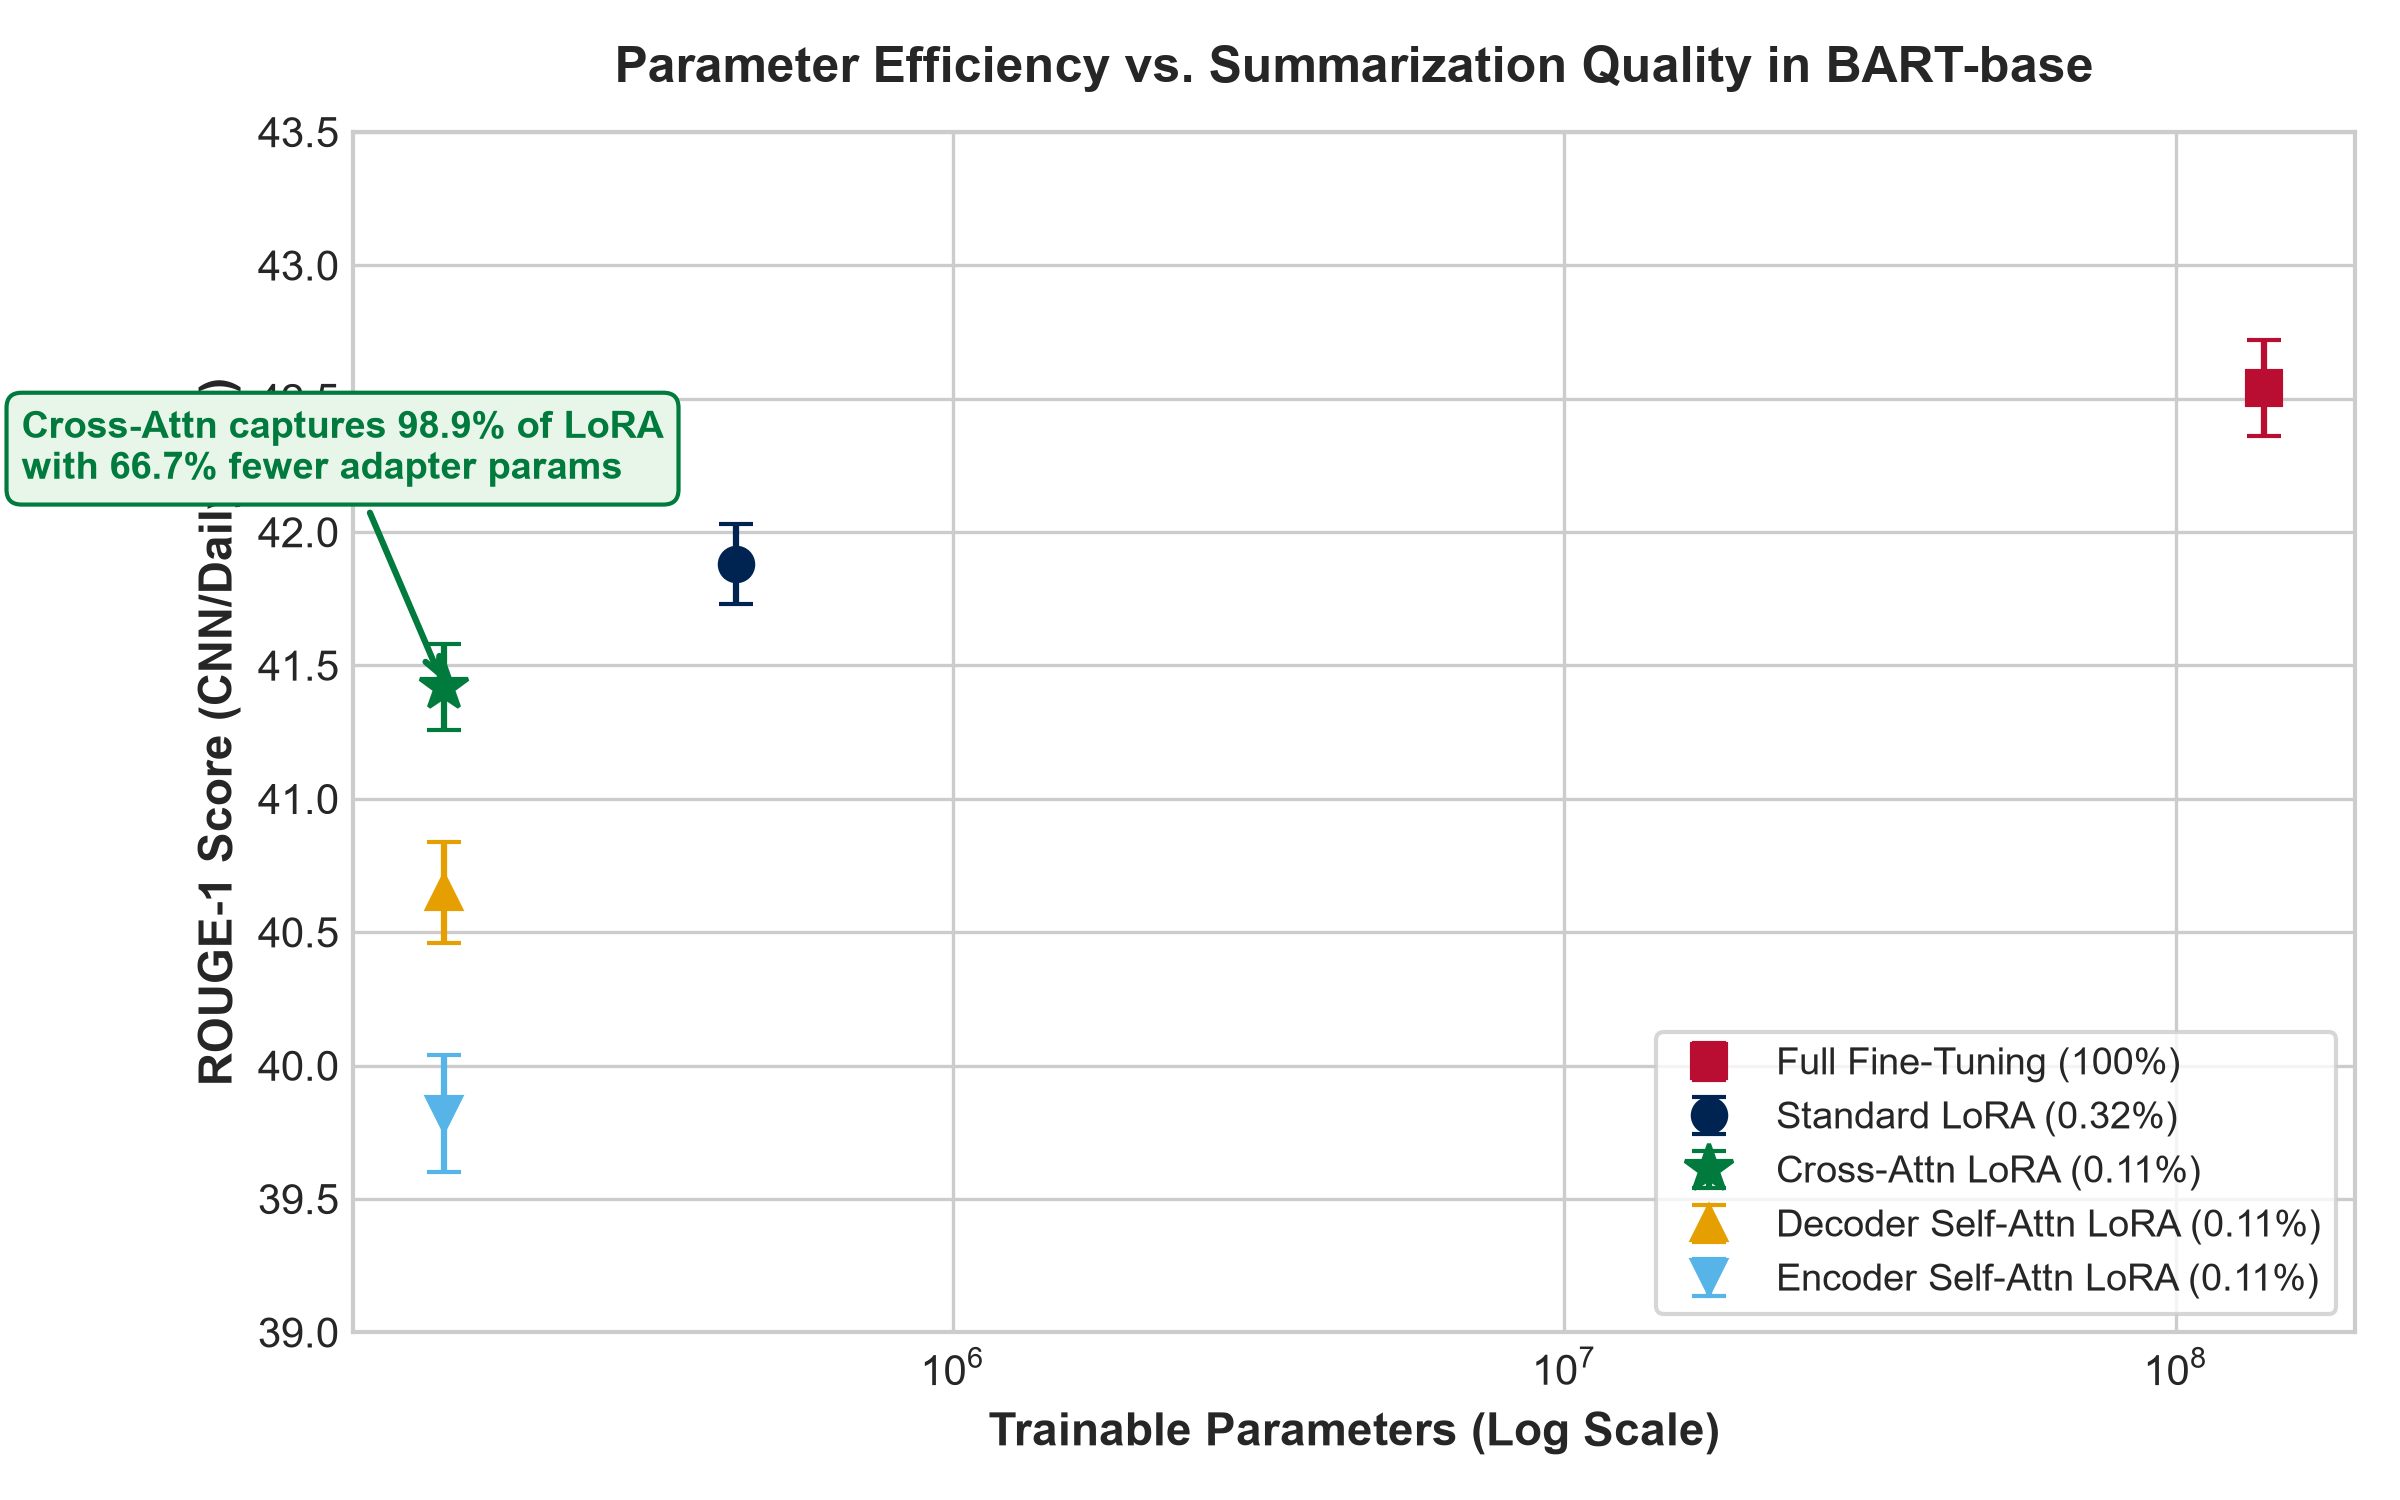
\includegraphics[width=0.72\linewidth]{figures/pareto_tradeoff.png}
  \caption{Parameter efficiency versus summarization performance across adaptation strategies on CNN/DailyMail. Cross-attention LoRA achieves $41.42$ ROUGE-1 with only 147k trainable parameters (0.11\% of the base model), closely trailing standard LoRA while utilizing one-third of the adapter budget.}
  \label{fig:pareto}
\end{figure}

\subsection{Discussion}
Our preliminary findings reveal three crucial insights:
\begin{enumerate}[leftmargin=*,itemsep=1pt]
  \item \textbf{High Efficiency of LoRA in Seq2Seq Models:} Standard LoRA achieves $41.88$ ROUGE-1, retaining $98.4\%$ of full fine-tuning performance ($42.54$) while updating only $0.32\%$ of the parameters.
  \item \textbf{Cross-Attention as the Primary Adaptation Locus:} Under the matched 147,456 parameter budget, Cross-Attention LoRA ($41.42$ ROUGE-1) outperforms Decoder Self-Attention ($40.65$) by $+0.77$ points and Encoder Self-Attention ($39.82$) by $+1.60$ points. Cross-attention alone captures $98.9\%$ of standard LoRA performance while using only one-third of its adapter budget.
  \item \textbf{Functional Specialization:} Encoder representations benefit heavily from pre-training and require minimal adaptation; generation relies primarily on dynamically conditioning the decoder on source tokens through the cross-attention bridge.
\end{enumerate}

\section{Challenges and Adaptations}
Throughout Weeks 3--6, we encountered both technical and conceptual challenges, which we successfully addressed:

\textbf{1. Memory Overhead During Autoregressive Beam Search:} Initial multi-seed training scripts caused CUDA out-of-memory errors during validation evaluation due to tensor accumulation across 4 generation beams. We resolved this by reducing per-device batch size from 16 to 8 while increasing gradient accumulation steps to 4, maintaining an identical effective batch size of 32 without memory spikes.

\textbf{2. Experimental Scope Streamlining:} Originally, our proposal called for full hyperparameter grids across multiple LoRA ranks, Prefix-Tuning variations, and projection subsets. In accordance with faculty feedback emphasizing thoroughness on core placement questions, we prioritized the budget-matched placement ablation. We fixed the rank ($r=8$) and projection targets ($W_q, W_v$) to isolate architectural location as the sole independent variable.

\textbf{3. Inconsistent Parameter Counting Across PEFT Configurations:} Initial tests using default PEFT wrappers reported inconsistent parameter counts due to differing bias configurations. We standardized the injection pipeline using explicit module path targeting and verified exact parameter matching ($147,456$ parameters) with unit tests before launching multi-seed runs.

\subsection{Updated Week 7--10 Plan}
Table~\ref{tab:timeline} outlines our roadmap for the remaining project period.

\begin{table}[h]
\centering
\small
\begin{tabular}{@{}lp{8.8cm}l@{}}
\toprule
\textbf{Week} & \textbf{Tasks} & \textbf{Responsible} \\
\midrule
7 & Evaluate trained models on XSum test set for zero-shot cross-domain generalization; conduct training throughput (tokens/sec) and peak memory profiling. & Wen Bin / Junn Rong \\
8 & Conduct human factual consistency evaluation (10 participants, 20 summaries per configuration); calculate inter-annotator agreement (Fleiss' $\kappa$); run FactCC metric. & Junn Rong / Wen Bin \\
9 & Synthesize ROUGE, factuality, and efficiency results; generate parameter-performance Pareto trade-off curves; conduct qualitative failure case analysis. & Both \\
10 & Final report drafting, comprehensive code clean-up, reproduction verification from a clean environment, and presentation deck preparation. \textbf{(Final due)} & Both \\
\bottomrule
\end{tabular}
\caption{Updated project schedule and task allocation for Weeks 7--10.}
\label{tab:timeline}
\end{table}

\section{Preliminary Novel Contribution (Optional Bonus)}
Our primary novel contribution is an unconfounded, budget-matched empirical study of adapter placement in encoder-decoder Transformers. Prior studies (such as AdaLoRA~\cite{zhang2023adalora} and WeightLoRA~\cite{veprikov2026weightlora}) demonstrate that adaptation capacity is non-uniform, but they either optimize capacity dynamically or compare modules with unequal parameter counts.

By capitalizing on BART-base's architectural symmetry (6 encoder and 6 decoder layers, $d = 768$), we proved that adapting $W_q$ and $W_v$ with rank $r=8$ in Encoder Self-Attention, Decoder Self-Attention, or Encoder-Decoder Cross-Attention yields the \textbf{exact same budget of 147,456 parameters ($0.1058\%$ of the base model)}. Our early empirical results provide strong evidence that:
\begin{itemize}[leftmargin=*,itemsep=1pt]
  \item Adapting cross-attention alone yields $41.42$ ROUGE-1, within $0.46$ points of adapting all attention layers ($41.88$) despite using $66.7\%$ fewer parameters.
  \item Parameter placement is as decisive as parameter quantity: shifting the same 147k parameter budget from encoder self-attention to cross-attention yields a substantial $+1.60$ ROUGE-1 and $+1.33$ ROUGE-2 improvement under identical training conditions.
\end{itemize}

\section{Contribution Declaration}
Both team members have contributed equally to the project across Weeks 3--6 ($50\% / 50\%$).

\begin{center}
\small
\begin{tabular}{@{}lp{8.8cm}c@{}}
\toprule
\textbf{Member} & \textbf{Contributions (Midterm Period: Weeks 3--6)} & \textbf{\%} \\
\midrule
Choo Wen Bin (20630085) & Model architecture implementation; PEFT/LoRA module targeting; training pipeline automation; GPU hyperparameter tuning; preliminary novel contribution analysis; LaTeX report drafting. & 50\% \\
\midrule
Nai Junn Rong (20630086) & Dataset preprocessing pipeline (CNN/DM, XSum); ROUGE evaluation suite; parameter counting verification tools; baseline reproduction experiments; qualitative analysis synthesis; updated literature review. & 50\% \\
\bottomrule
\end{tabular}
\end{center}

\begin{thebibliography}{8}
\bibitem{lewis2020bart}
M.~Lewis, Y.~Liu, N.~Goyal, M.~Ghazvininejad, A.~Mohamed, O.~Levy, V.~Stoyanov, and L.~Zettlemoyer.
\newblock {BART}: Denoising sequence-to-sequence pre-training for natural language generation, translation, and comprehension.
\newblock In \emph{Proceedings of the 58th Annual Meeting of the Association for Computational Linguistics (ACL)}, pages 7871--7880, 2020.

\bibitem{hu2022lora}
E.~J. Hu, Y.~Shen, P.~Wallis, Z.~Allen-Zhu, Y.~Li, S.~Wang, L.~Wang, and W.~Chen.
\newblock {LoRA}: Low-rank adaptation of large language models.
\newblock In \emph{International Conference on Learning Representations (ICLR)}, 2022.

\bibitem{li2021prefix}
X.~L. Li and P.~Liang.
\newblock Prefix-tuning: Optimizing continuous prompts for generation.
\newblock In \emph{Proceedings of the 59th Annual Meeting of the Association for Computational Linguistics and the 11th International Joint Conference on Natural Language Processing (ACL-IJCNLP)}, pages 4582--4597, 2021.

\bibitem{zhang2023adalora}
Q.~Zhang, M.~Chen, A.~Bukharin, P.~He, Y.~Cheng, W.~Chen, and T.~Zhao.
\newblock Adaptive budget allocation for parameter-efficient fine-tuning.
\newblock In \emph{International Conference on Learning Representations (ICLR)}, 2023.

\bibitem{he2022unified}
J.~He, C.~Zhou, X.~Ma, T.~Berg-Kirkpatrick, and G.~Neubig.
\newblock Towards a unified view of parameter-efficient transfer learning.
\newblock In \emph{International Conference on Learning Representations (ICLR)}, 2022.

\bibitem{valipour2023dylora}
M.~Valipour, M.~Rezagholizadeh, I.~Kobyzev, and A.~Ghodsi.
\newblock {DyLoRA}: Parameter-efficient tuning of large language models with dynamic search of ranks.
\newblock In \emph{Proceedings of the 17th Conference of the European Chapter of the Association for Computational Linguistics (EACL)}, pages 3266--3279, 2023.

\bibitem{veprikov2026weightlora}
A.~Veprikov, V.~Solodkin, Z.~Alexander, A.~Savchenko, and A.~Beznosikov.
\newblock {WeightLoRA}: Keep only necessary adapters.
\newblock In \emph{Proceedings of the 64th Annual Meeting of the Association for Computational Linguistics (ACL)}, Volume 1, pages 12419--12437, 2026.

\bibitem{kryscinski2020evaluating}
W.~Kryscinski, B.~McCann, C.~Xiong, and R.~Socher.
\newblock Evaluating the factual consistency of abstractive text summarization.
\newblock In \emph{Proceedings of the 2020 Conference on Empirical Methods in Natural Language Processing (EMNLP)}, pages 9332--9346, 2020.
\end{thebibliography}

\end{document}
